\chapter{chapter 1 title}

Aenean malesuada tincidunt quam, ut dapibus nunc fermentum porta. Donec euismod auctor laoreet. Pellentesque euismod enim et orci tempor, eget posuere nisi aliquet. Integer posuere tristique sem eu vehicula. Integer eget odio et mauris tincidunt viverra. Donec euismod tortor congue magna lacinia, ac accumsan arcu dignissim. Cras non diam eget mi ultricies laoreet quis eu odio. Suspendisse eu iaculis erat, at ornare nisi. Etiam ut neque ligula. Nam luctus orci a nulla vulputate, eget vestibulum nunc vulputate. Quisque at arcu auctor, maximus velit pretium, pulvinar nisi. In eu finibus augue. Aliquam ligula diam, tempus id nibh at, condimentum convallis quam. Sed a leo non tortor aliquam venenatis.


\section{sec 1}
Aenean malesuada tincidunt quam, ut dapibus nunc fermentum porta. Donec euismod auctor laoreet. Pellentesque euismod enim et orci tempor, eget posuere nisi aliquet. Integer posuere tristique sem eu vehicula. Integer eget odio et mauris tincidunt viverra. Donec euismod tortor congue magna lacinia, ac accumsan arcu dignissim. Cras non diam eget mi ultricies laoreet quis eu odio. Suspendisse eu iaculis erat, at ornare nisi. Etiam ut neque ligula. Nam luctus orci a nulla vulputate, eget vestibulum nunc vulputate. Quisque at arcu auctor, maximus velit pretium, pulvinar nisi. In eu finibus augue. Aliquam ligula diam, tempus id nibh at, condimentum convallis quam. Sed a leo non tortor aliquam venenatis.

\section{sec 2}
Aenean malesuada tincidunt quam, ut dapibus nunc fermentum porta. Donec euismod auctor laoreet. Pellentesque euismod enim et orci tempor, eget posuere nisi aliquet. Integer posuere tristique sem eu vehicula. Integer eget odio et mauris tincidunt viverra. Donec euismod tortor congue magna lacinia, ac accumsan arcu dignissim. Cras non diam eget mi ultricies laoreet quis eu odio. Suspendisse eu iaculis erat, at ornare nisi. Etiam ut neque ligula. Nam luctus orci a nulla vulputate, eget vestibulum nunc vulputate. Quisque at arcu auctor, maximus velit pretium, pulvinar nisi. In eu finibus augue. Aliquam ligula diam, tempus id nibh at, condimentum convallis quam. Sed a leo non tortor aliquam venenatis.

...

Figure \ref{sample1} shows lab lab lah
\begin{figure}[ph!]
\psfrag{XL}[][][0.75][0]{$x$}
\psfrag{YL}[][][0.75][0]{$y$}
\psfrag{S1}[][][0.75][0]{a circle}
\psfrag{S2}[][][0.75][0]{a star}
\centering
\subfigure[]{\label{} 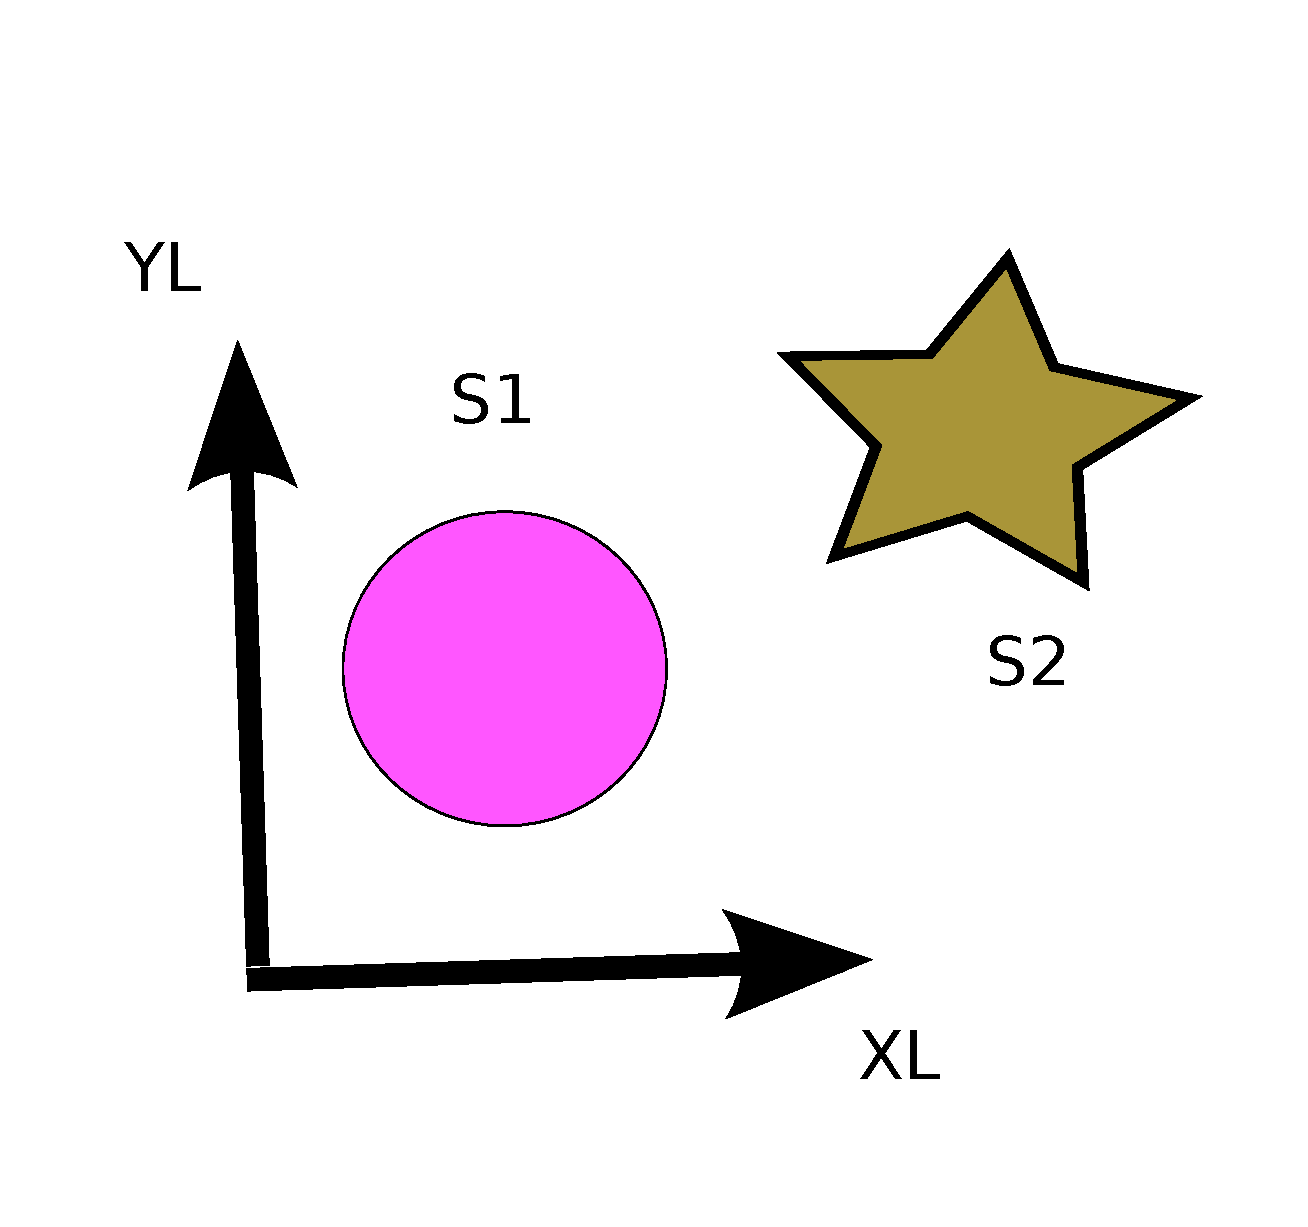
\includegraphics[width=0.35\textwidth]{paper_1_fig_1}}
\subfigure[]{\label{} 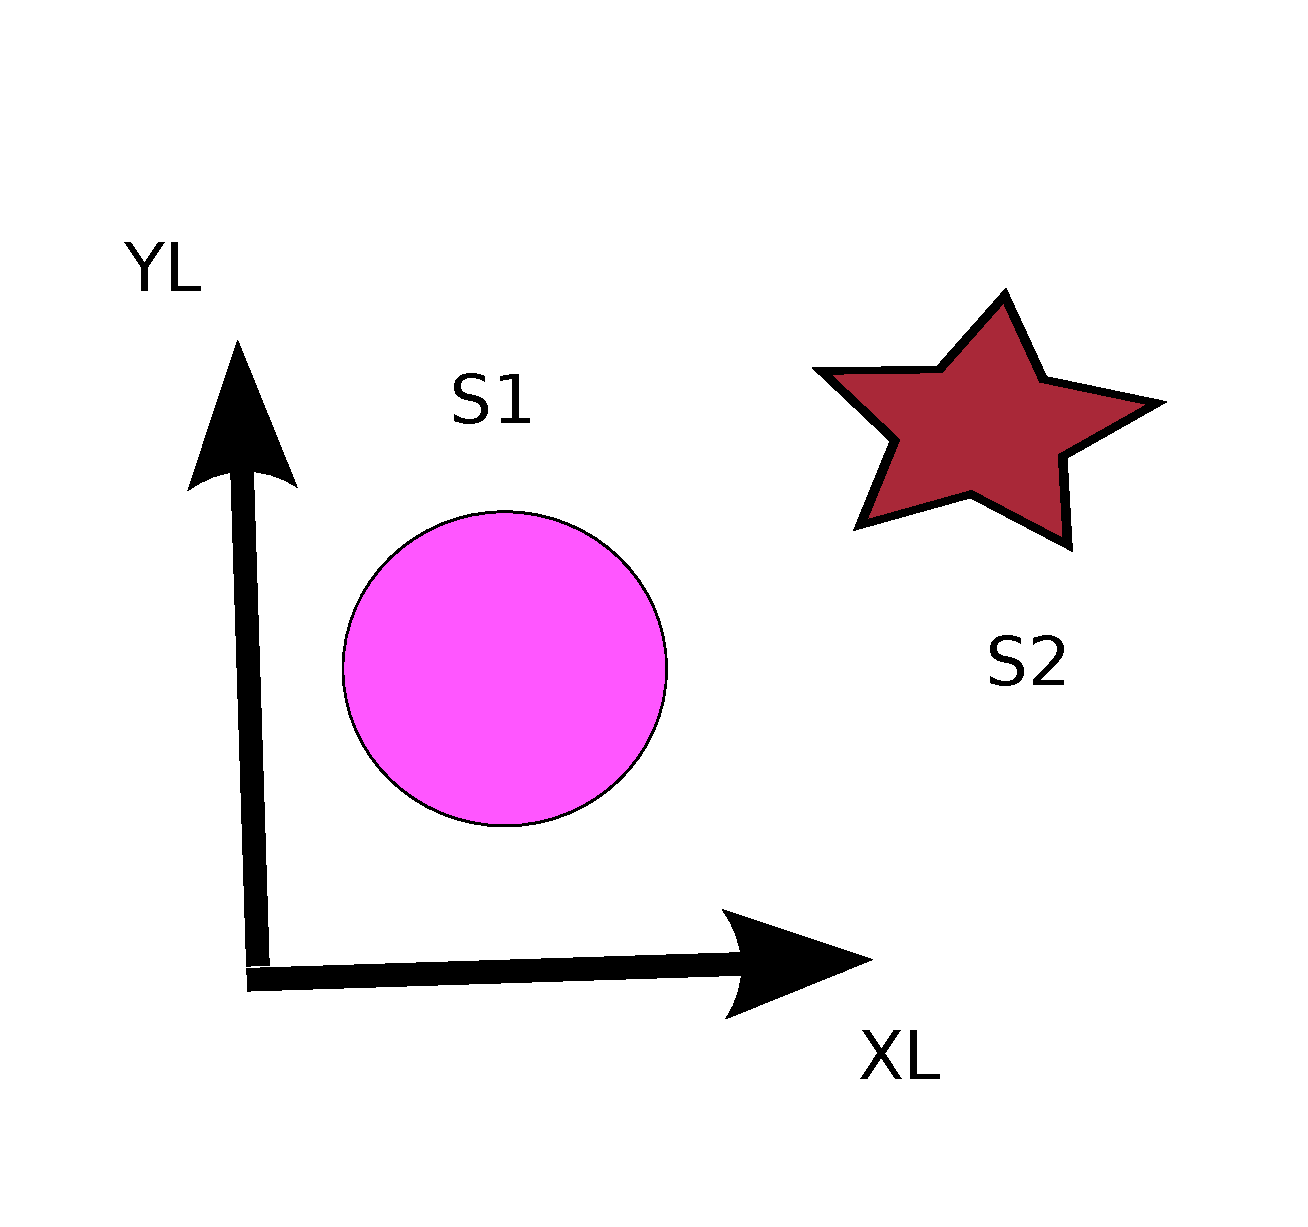
\includegraphics[width=0.35\textwidth]{paper_1_fig_2}} \\
\caption{\label{sample1} This is a sample figure that uses the ``psfrag'' package [https://en.wikipedia.org/wiki/PSfrag]. This package is very useful because it can replace predefined labels in the eps figures with latex commands. The only draw-back is that it does not work with pdfLatex. So to get a final pdf you have to make a ps first and then convert it to pdf {the steps to this are latex->dvi2ps->ps2pdf}. Usually the implementation of the latex come from executables for doing the operations shown in the curly braces. (a) shows something and (b) shows something else.} 
\end{figure}


Figure \ref{sample2} is another figure sample 
\begin{figure}[ph!]
\centering
\subfigure[]{\label{} 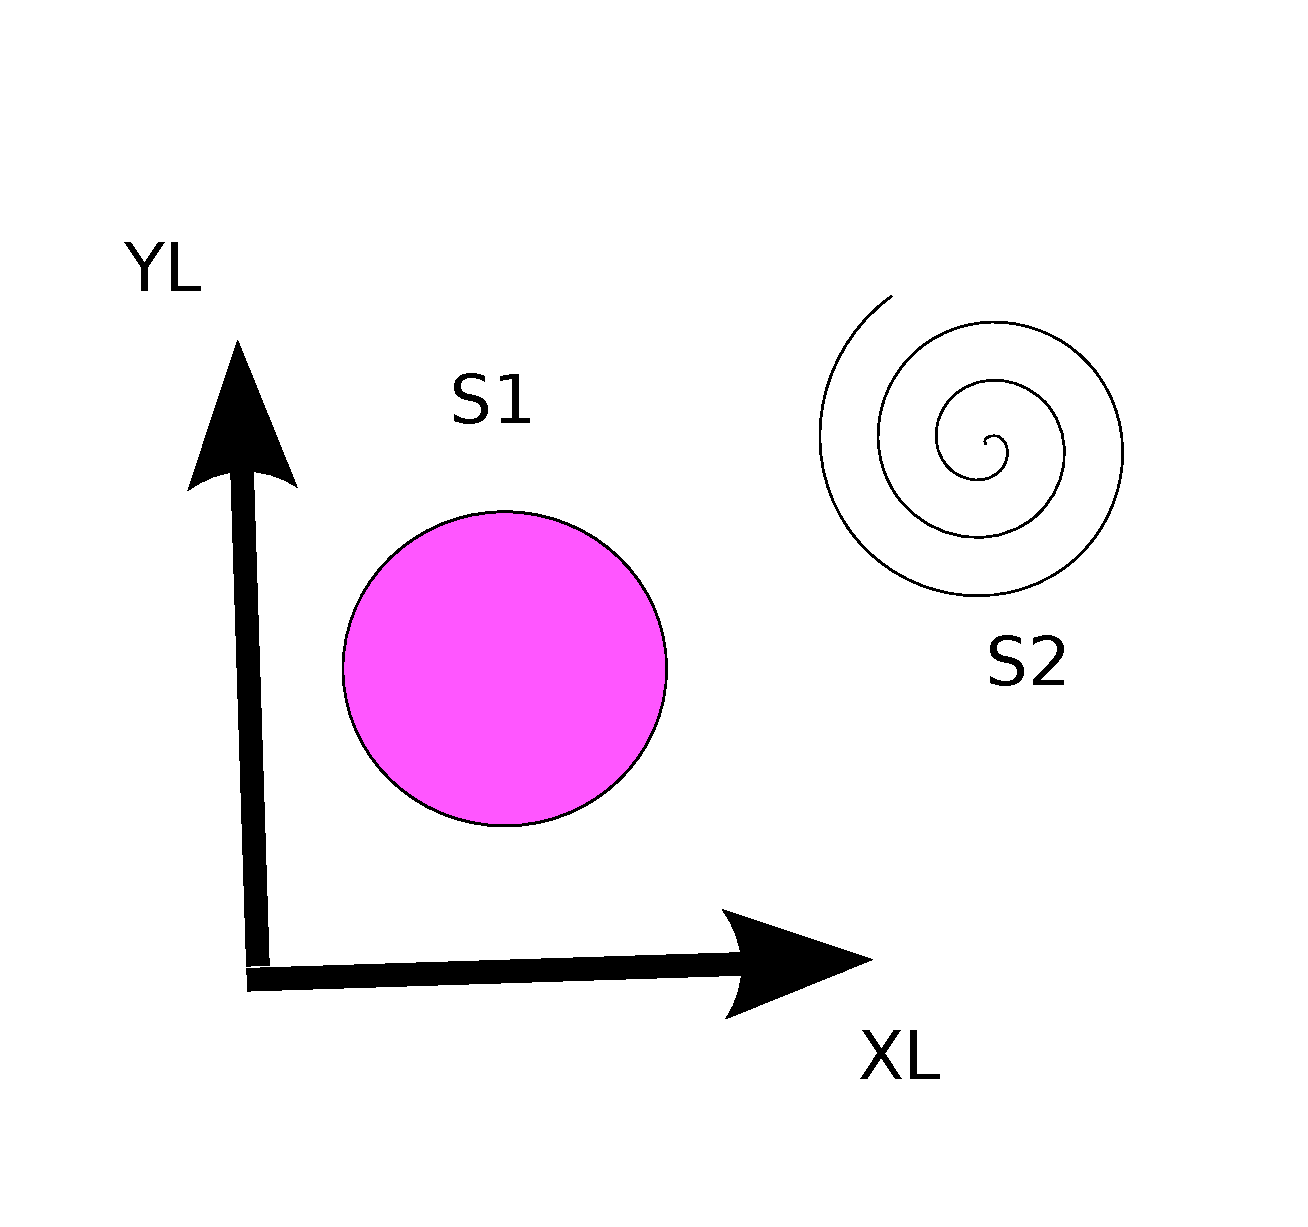
\includegraphics[width=0.35\textwidth]{paper_2_fig_1}}
\subfigure[]{\label{} 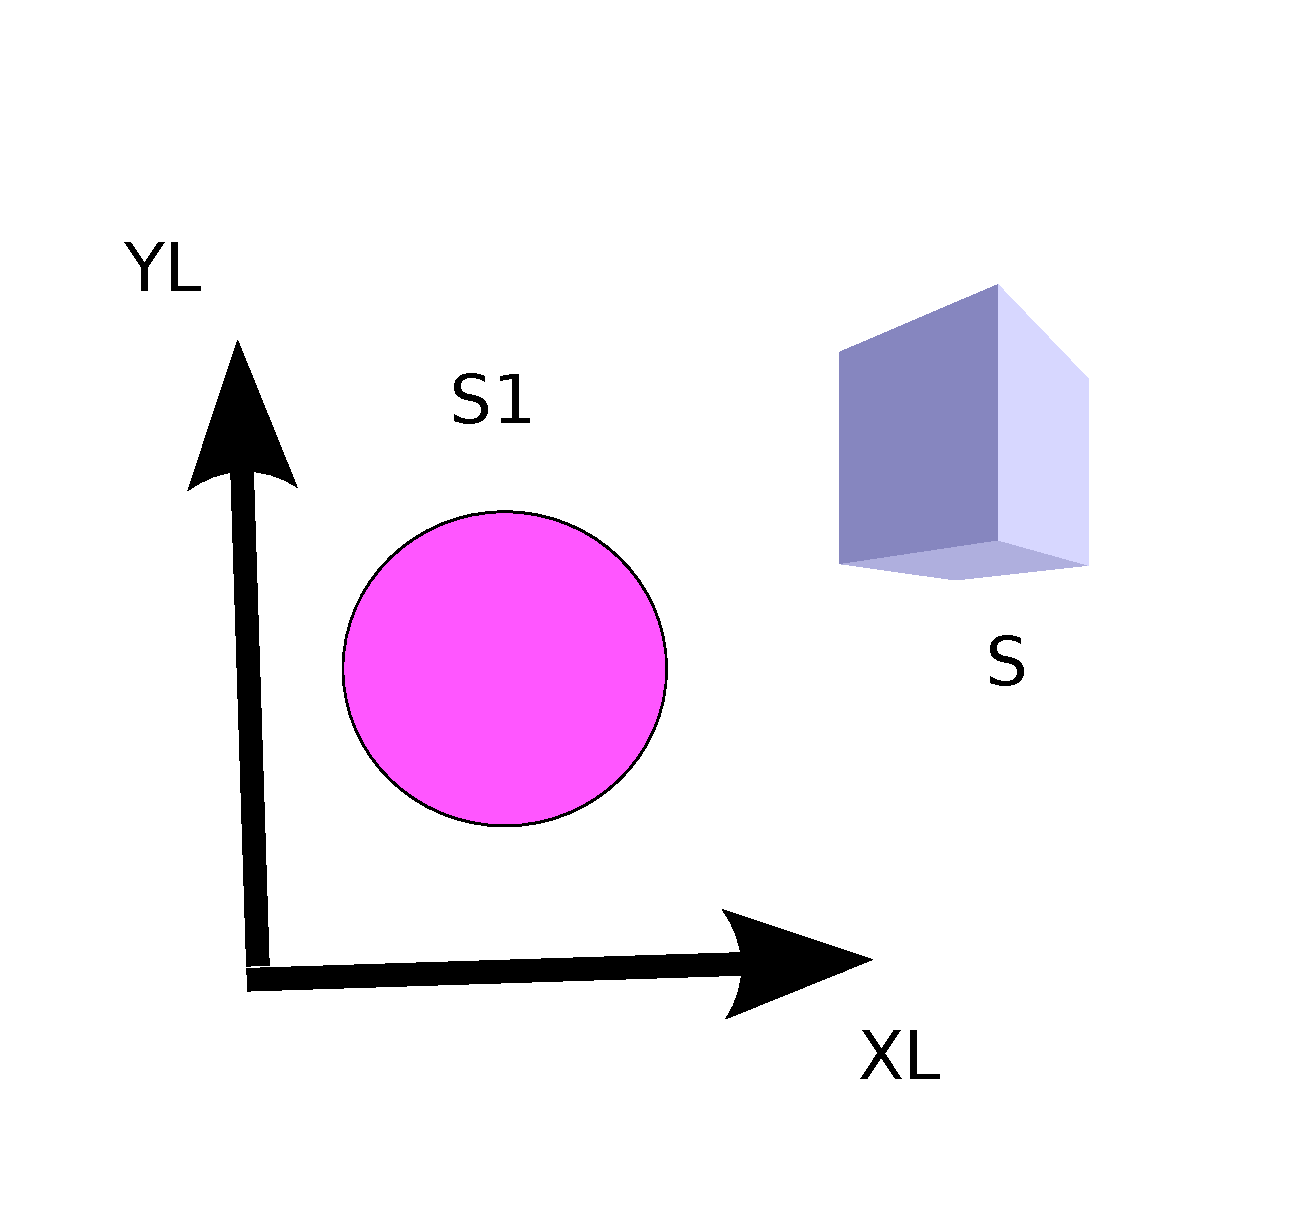
\includegraphics[width=0.35\textwidth]{paper_2_fig_2}} \\
\caption{\label{sample1} This is a sample figure that does not use the ``psfrag'' package [https://en.wikipedia.org/wiki/PSfrag], and therefore original labels in the eps files are shown. (Note that you can open the eps files with a text editor and search for the corresponding labels in it, and changes the labels, if you want to, form within the eps file.)  a) shows something and (b) shows something else.} 
\end{figure}

